
\subsection{Banco de pruebas}


Para poder realizar pruebas del SAL/T fue necesario armar un banco de pruebas con componentes, módulos y sistemas externos que permitan simular las condiciones de operación real. En la figura \ref{fig:testbench} se visualiza el banco de pruebas completo que se utilizó para realizar las pruebas del dispositivo. 


\begin{figure}[H]
    \centering
    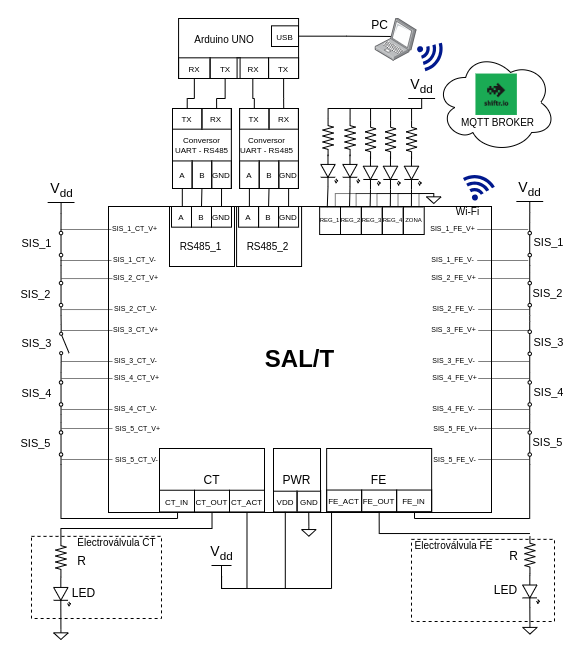
\includegraphics[width = \linewidth]{img/testbench.png}
    \caption{Banco de pruebas completo del SAL/T}
    \label{fig:testbench}
\end{figure}


Los buses de las señales de corte de tracción y freno de emergencia fueron representados cada uno con cinco llaves en serie donde cada una representa la llave de estado de cada SIS. El polo negativo de la llave del último SIS se conecta en la entrada del SAL/T CT\_IN (o FE\_IN para el otro bus). Luego, la salida CT\_OUT (o FE\_OUT) se conecta con la electroválvula correspondiente representada por una resistencia y un LED para visualizar su estado de activación. También se conectó la misma señal de activación que alimenta el bus a la entrada CT\_ACT (o FE\_ACT); en este banco de pruebas, se utilizó una tensión de 5 V para alimentar los buses porque facilitó la obtención de la fuente frente a una de 72 VDC o 110 VDC. Sin embargo, mediante el firmware se va a poder compensar esa diferencia en la tensión esperada luego del circuito de medición de los SIS modificando el umbral de los valores esperados en el ADC para determinar si una llave está abierta o cerrada. Por lo tanto, con este esquema se va a poder representar de una manera bastante similar al de operación real, el bus en serie de los SIS que termina en una electroválvula y la intención del SAL/T de intervenir y forzar estados luego de la posible apertura de la línea por alguno de los SIS. \\

Respecto a las salidas de registro de estado del SAL/T y al conector de zona, que permiten la conexión de baja o alta impedancia entre sus dos terminales dependiendo el estado a reportar, se conectó una resistencia y un LED en un terminal, y conexión a tierra en el otro. Esto se replicó en cada uno de los conectores para poder visualizar el estado reportado a la formación para cada una de las salidas. \\ 


Para simular las comunicaciones con los sistemas de medición de velocidad, se utilizó un Arduino Uno \cite{arduino_uno} y dos módulos conversores UART - RS-485 \cite{conversor_rs485}. El Arduino Uno es una placa de desarrollo basada en el microcontrolador ATmega328P \cite{atmega328}. Cuenta con 14 pines digitales, 6 entradas analógicas, un único puerto UART para comunicación serie, y funciona a 5 V con una frecuencia de reloj de 16 MHz. Incluye una interfaz USB para la programación y alimentación, junto con un puerto de alimentación externa. Si bien el Arduino Uno cuenta solo con una interfaz UART, se puede simular una segunda utilizando la librería SoftwareSerial \cite{swSerial} que obtiene resultados suficientes cuando no es necesario realizar una comunicación bidireccional. En la figura \ref{fig:arduino_uno} se visualiza la placa Arduino Uno utilizada. 

\begin{figure}[H]
    \centering
    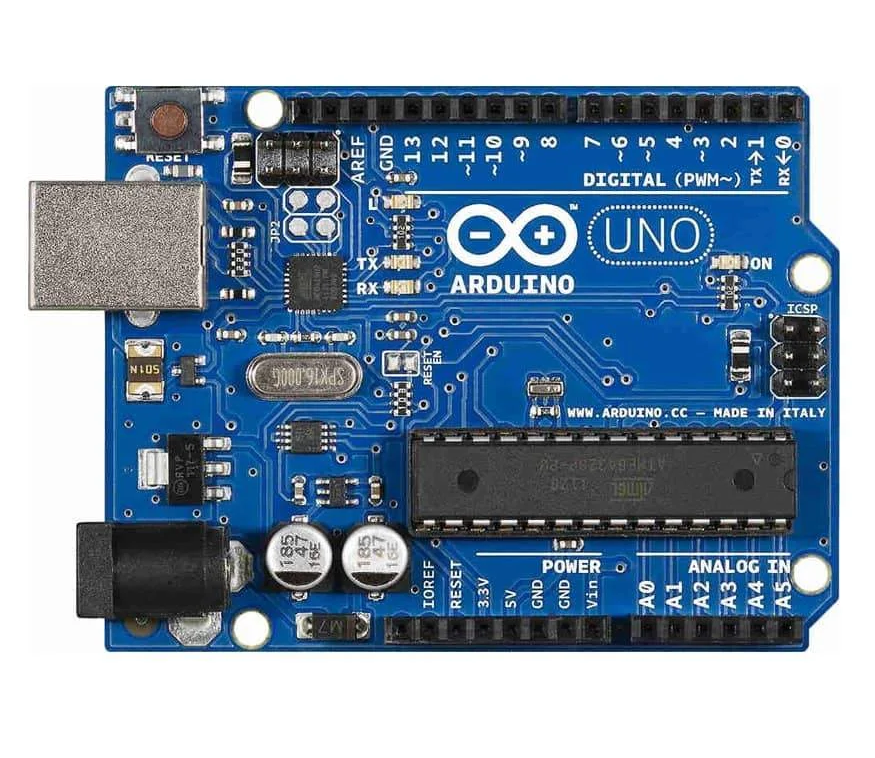
\includegraphics[width = 0.6 \linewidth]{img/arduino_uno.png}
    \caption{Placa de desarrollo Arduino Uno}
    \label{fig:arduino_uno}
\end{figure}


El módulo conversor UART - RS-485 utilizado se puede visualizar en la figura \ref{fig:conversor_uart_rs485}; es un módulo fabricado por Hobbytrónica \cite{hobbytronica} basado en el chip MAX485 \cite{max485}; un transceptor de bajo consumo que permite la comunicación serial diferencial a través del protocolo RS-485. Este módulo tiene entradas para el lado de la comunicación UART (TX, RX) y un selector para habilitar la transmisión o la recepción, ya que al pasar a RS-485, se convierte en una comunicación half-duplex. Por el lado del RS-485, tiene las salidas de A y B esperadas. 


\begin{figure}[H]
    \centering
    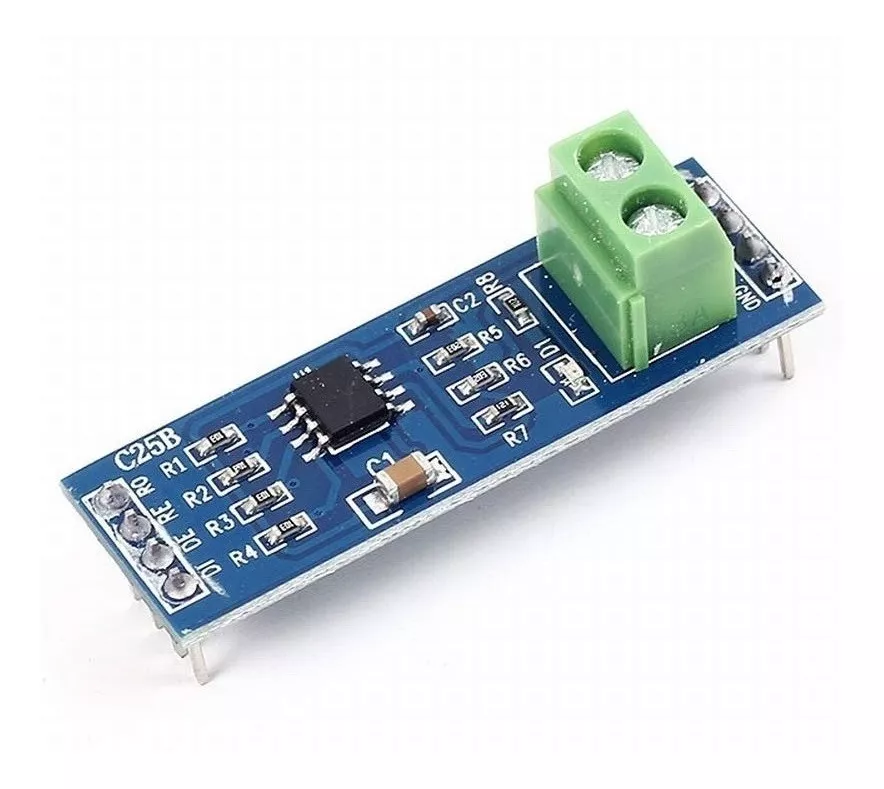
\includegraphics[width = 0.5\linewidth]{img/conversor_uart_rs485.png}
    \caption{Módulo conversor UART a RS-485}
    \label{fig:conversor_uart_rs485}
\end{figure}

El Arduino va a simular en una de sus interfaces la señal proveniente del Hasler Teloc 1500 generada tramas de 31 bytes iniciadas y terminadas por un byte de start/stop 0x7E y con la información de velocidad en los bytes 7 y 8. En la otra de sus interfaces va a comunicar el valor numérico de la velocidad que transmitiría el circuito de adaptación e interpretación del generador de impulsos ópticos. Ambas interfaces van a emitir comunicaciones continuas cada 1 segundo con el último valor configurado. \\ 

Por otro lado, el Arduino va a estar conectado a una PC por el conector USB y, mediante comunicación serie, va a estar recibiendo los datos de velocidad a transmitir en cada una de sus interfaces. De esta manera, se puede ir variando las velocidades reportadas al SAL/T en cada una de sus interfaces en todo momento desde una PC. \\ 


La PC también va a simular las interacciones de la central operativa conectada al broker MQTT generado con la plataforma shiftr.io \cite{shifrio}; una plataforma en línea que permite visualizar y gestionar flujos de datos en tiempo real mediante el protocolo MQTT. Proporciona un panel interactivo donde se pueden ver en vivo los mensajes publicados y suscritos entre dispositivos, facilitando el monitoreo y depuración de redes IoT. Es fácil de usar y ofrece herramientas para desarrollar, probar y supervisar la comunicación entre dispositivos conectados. Por lo tanto, la PC va a poder enviar comandos remotos al SAL/T a través del broker MQTT y al mismo tiempo va a recibir los mensajes de confirmación de recepción (ACK), los logs del sistema y el reporte periódico del estado del sistema. El SAL/T está configurado para interactuar con el mismo broker MQTT conectándose al servidor a través de la red Wi-Fi que le permite conectarse al módulo interno ESP32. En la figura \ref{fig:shiftrio}
se visualiza el broker shiftr.io con el SAL/T y la central operativa conectados y suscriptos a los distintos \textit{topics} MQTT intercambiando mensajes.



\begin{figure}[H]
    \centering
    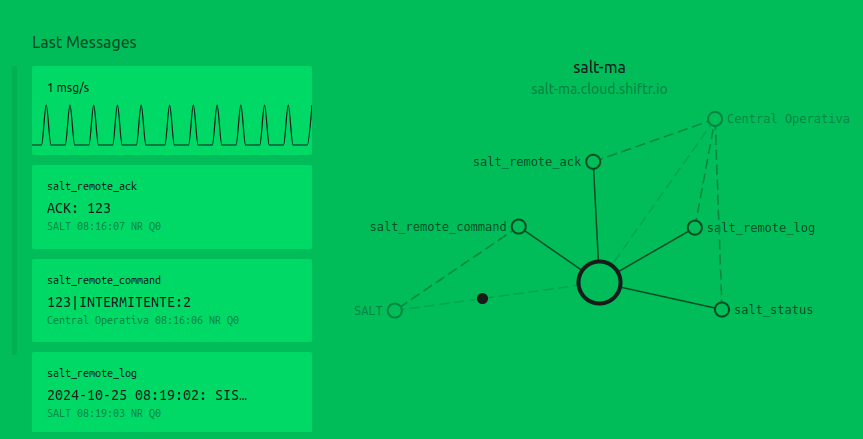
\includegraphics[width = \linewidth]{img/shiftrio.png}
    \caption{Visualización de shifr.io conectando el SAL/T con la central operativa}
    \label{fig:shiftrio}
\end{figure}






